\documentclass[10pt,journal,letterpaper]{IEEEtran}
\usepackage{pgfplots}
\pgfplotsset{/pgfplots/ybar legend/.style={
        /pgfplots/legend image code/.code={%
            \draw[##1,/tikz/.cd,yshift=-0.25em]
            (0cm,0cm) rectangle (3pt,0.75em);},
    },
}
\usepackage{caption}
\usepackage{booktabs}
\usepackage{tikz}
\usepackage{enumerate}
\usepackage{xcolor,cite}
\usepackage{pdflscape}
\usepackage{graphicx}
\usepackage{adjustbox}
\usepackage[outdir=./]{epstopdf}
\usepackage{amsmath,amssymb}
\usepackage[english]{babel}
\usepackage[applemac]{inputenc}
\usepackage{mathptmx}
\usepackage[flushleft]{threeparttable}
\usepackage[font=small,skip=3pt]{caption}
\usepackage{url}
\usepackage{xcolor}
\usepackage{caption}
\usepackage[ruled,vlined]{algorithm2e}
\usepackage{multirow}
\usepackage{multicol}
\usepackage{moreverb}
\usepackage{fix-cm}
\usepackage{subcaption}
\usepackage{enumitem}
\newtheorem{dfn}{Definition}
\newtheorem{proof}{Proof}
\newtheorem{theorem}{Theorem}

% \definecolor{bblue}{HTML}{4F81BD}
% \definecolor{rred}{HTML}{C0504D}
% \definecolor{ggreen}{HTML}{9BBB59}
% \definecolor{ppurple}{HTML}{9F4C7C}

\begin{document}
\title{ID-CPPA-CBA: Provably Secure Identity-based Conditional Privacy-preserving Authentication and Clustering-based Batch Verification for VANETs}

\author{SK Hafizul Islam, \emph{Senior~Member,~IEEE},~Hrithik~Kumar,~Aditya~S.~Gudimetla,~Rohan~Chakraborty
\IEEEcompsocitemizethanks{\IEEEcompsocthanksitem S. H. Islam and H.
Kumar, A. S. Gudimetla, and R. Chakraborty are with the Department
of Computer Science and Engineering, Indian Institute of Information
Technology Kalyani, West Bengal 741235, India. \protect E-mail:
hafi786@gmail.com, hritrak@gmail.com, adityagudimetla@gmail.com,
chakrabortyrohan34@gmail.com}
\thanks{}}

\IEEEcompsoctitleabstractindextext{

\begin{abstract}
In this paper, we have proposed conditional privacy-preserving
authentication scheme, for secure Vehicle-to-Infrastructure (V2I)
communication in Vehicular Ad Hoc Networks (VANETS). We use
pseudo-identity for this purpose and it facilitates the Trusted
Authorities (TAs) to track the real-identity of a vehicle by its
signature but not any malicious user. In our proposed scheme, we
used the clustering technic to speedup the batch verification
process to simultaneously verify all the authentication messages
send by a number of vehicles. A new protocol in batch verification
is also proposed, called clustering which allows the vehicles to
help a Road-Side Unit (RSU) in the verification process.
\end{abstract}

\begin{IEEEkeywords}
Authentication, Batch verification, Binary search, Bilinear pairing,
Clustering, Digital signature,
\end{IEEEkeywords}}
\maketitle


\IEEEdisplaynotcompsoctitleabstractindextext
\IEEEpeerreviewmaketitle

\vspace{-0.25cm}

\section{Introduction}
In recent years, the rise of self-driving vehicles and dedicated
short-range communications technologies have led to an increase in
Vehicular Ad Hoc Networks (VANETs). A VANET is considered as a
particular type of Mobile Ad Hhoc Network (MANET). They share some
similarities, such as their rapidly and dynamically changing network
topologies due to the fast motion of vehicles; however, they do have
specific vital differences in both architecture and design\textcolor{blue}{\cite{r16}}. The mobility of
vehicles in VANETs is, in general, constrained by predefined roads.
Various conditions, such as road conditions, weather situations,
traffic, and traffic control mechanisms (stop signs, traffic lights,
and speed limits), restrict the velocity of a vehicle. Besides,
given the fact that vehicles can be equipped with devices with
potentially longer transmission ranges, rechargeable source of
energy, and extensive onboard storage capacities, processing power,
and storage efficiency are not an issue in VANETs as they are in
MANETs\textcolor{blue}{ \cite{r16}} . From
these features, VANETs are considered as an extremely flexible and
relatively easy-to-manage network pattern of MANETs.

VANET applications include onboard active safety systems that are
used to assist drivers in avoiding collisions and in coordinating
among them at critical points, such as intersections and highway
entries \textcolor{blue}{\cite{r17}}.
Safety systems may intelligently disseminate road information, such
as incidents, real-time traffic congestion, high-speed tolling, or
surface condition to vehicles in the vicinity of the subjected
sites. This helps to avoid platoon vehicles and to improve road
capacity accordingly \textcolor{blue}{\cite{r17}}. With such active safety systems, the number of vehicle
accidents and associated damage are expected to be largely reduced.
In addition to the safety, as mentioned above applications, IVC
\textcolor{blue}{(Inter-Vehicicular-Communication, or V-2-V i.e. Vehicle-to-Vehicle comm.)\cite{r18}} communications can also be used to
provide comfort applications. The latter may include weather
information, gas station, restaurant locations, mobile e-commerce,
entertainment applications, and interactive communications such as
Internet access, music downloads, and content delivery \cite{r15}.


\subsection{System model}\label{L111}
The two-layer network model is very suitable for VANETs \cite{r7}.
The various components of the network model are shown in
Fig.~\ref{fig1(model)}. The top layer of the network model is
comprised of traffic control centers (TCCs), and Trusted Authorities
(TAs), where they could communicate with each other securely through
the Secure Socket Layer (SSL) protocol. The bottom layer of the
network model consists of a number of Road-Side-Units (RSUs) and
vehicles, where they could communicate with each other through the
Dedicated Short Range Communication (DSRC) protocol\textcolor{blue}{\cite{r19}}. The details of the
participants of the network model are given as follows:
\begin{itemize}
\item \textbf{Trusted Authority (TA):}~The TAs and the PKG are always
trusted and can never be compromised, and two or more TAs do not
collude. They are also powered with sufficient computation and
storage capabilities. A TA is responsible for generating system
parameters and preloading them in the OBU of the vehicle offline. It
is the only participant that could get the real identity of the
vehicle from the intercepted messages.
\item \textbf{Road-Side Unit (RSU):}~A RSU is a wireless communication
device that uses a DSRC protocol. It is located on the roadside and
could communicate with the vehicles. It can verify the validity of
received messages and sends them to the traffic management center or
process them locally.
\item \textbf{Vehicle:}~A vehicle in a VANET equipped with a tamper-proof
device, called On-Board Unit (OBU).An OBU is a wireless
communication device, and its information is never be compromised.
Through a DSRC protocol, an OBU helps a vehicle to exchange traffic
information with the nearby vehicles, RSUs, and can also communicate
with the TCC via the Internet. Each vehicle in a VANET has its own
real identity, pseudo-identity, and a private key. A vehicle used
its private key to sign all the messages and send them to a nearby
RSU. Each RSU that receives traffic-information is responsible for
verifying the digital signatures of the messages.
\end{itemize}
%%%%%%%%%%%%%%%%%%%%%%%%%%%%%%%%%%%%%%%%%%%%%%%%%%%%%%%%%%%%%%%%%%%%%%%
\begin{figure}[h]
    \centering
    \captionsetup{justification=centering}
    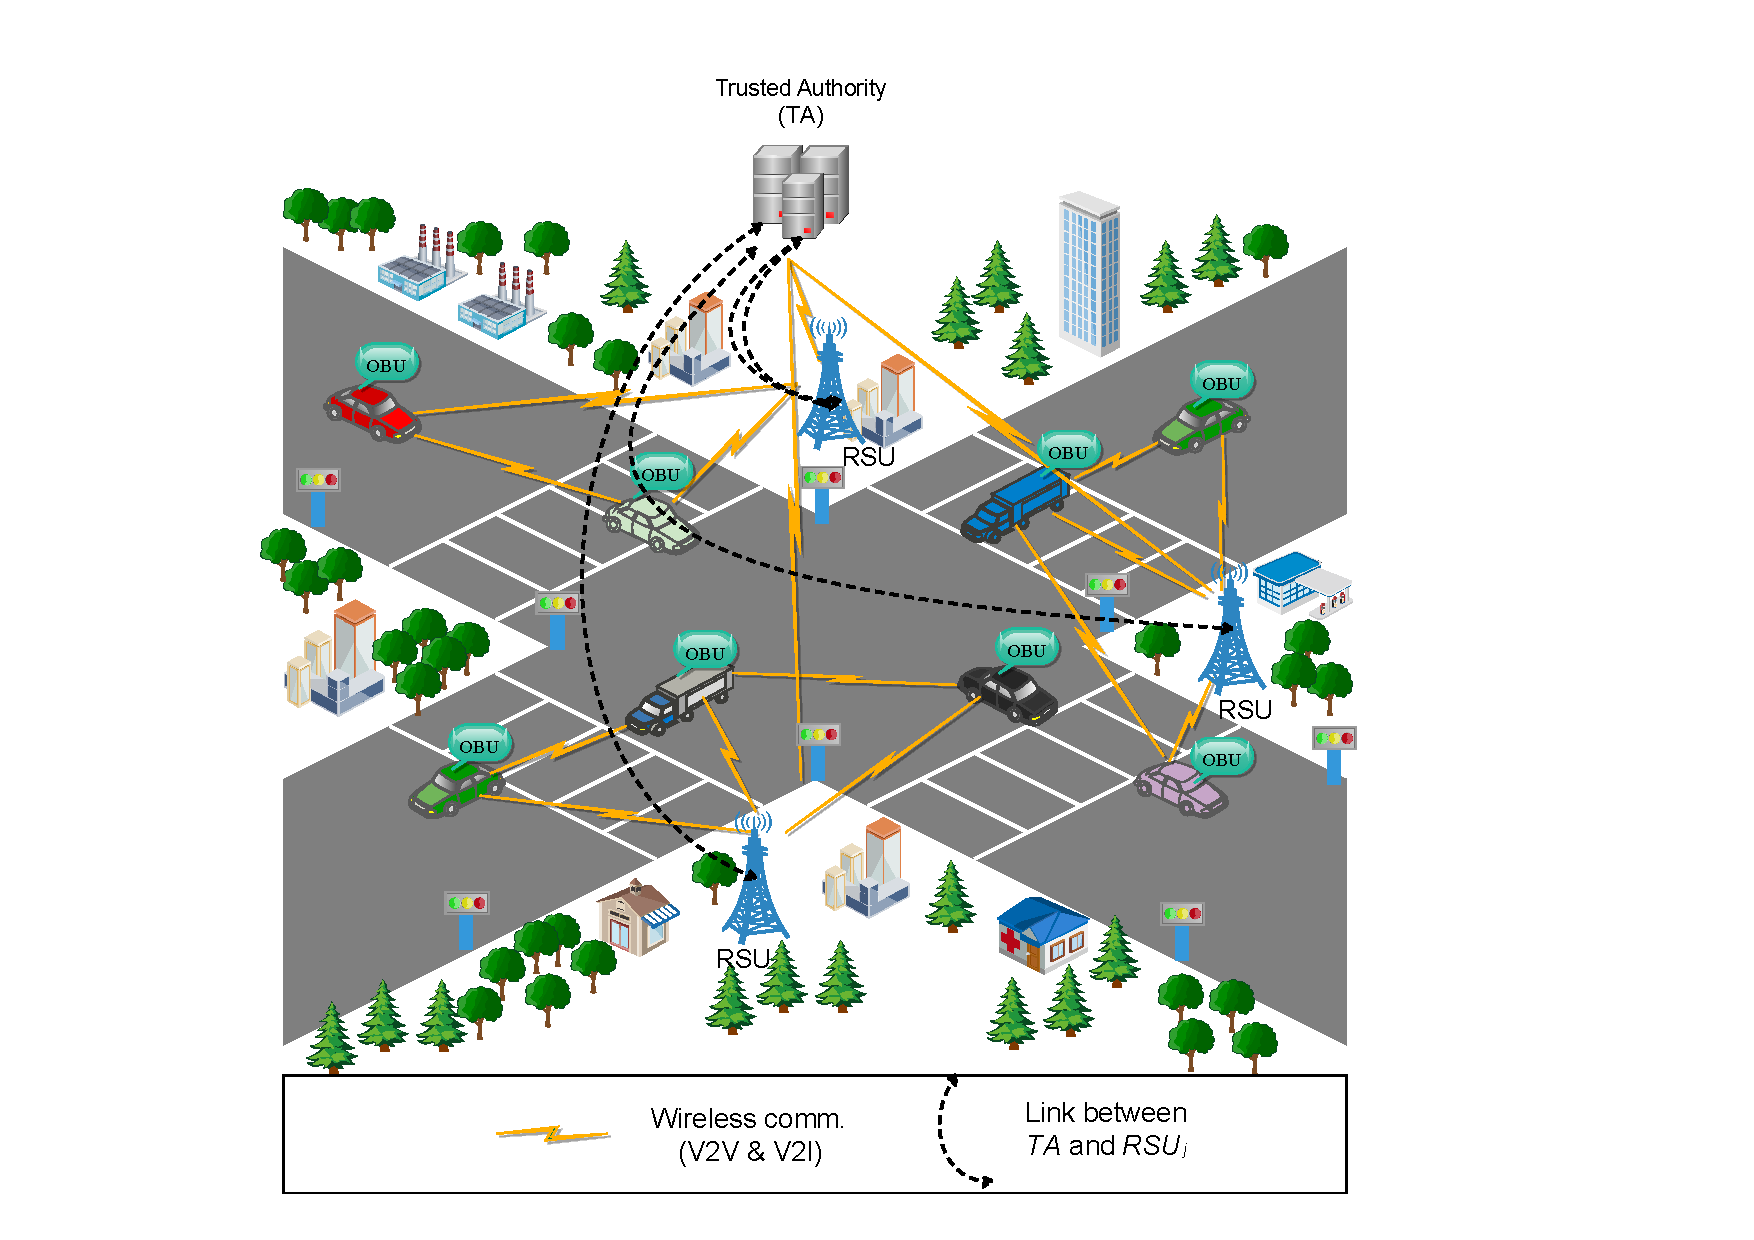
\includegraphics[scale=0.45]{Fig1(model).pdf}
    \caption{Two-layer network model for VANET}
    \label{fig1(model)}
\end{figure}
%%%%%%%%%%%%%%%%%%%%%%%%%%%%%%%%%%%%%%%%%%%%%%%%%%%%%%%%%%%%%%%%%%%%%%%
The RSUs communicate with an AS and a TA using a secure transmission
protocol, such as the wired Transport Layer Security (TLS) protocol.
The RSUs are responsible for forwarding the valid messages received
from the OBUs to an AS. A TCC is in charge of further analysis and
giving feedback to the RSUs after collecting traffic-related
information such as the current time, location, instances of traffic
accidents, traffic distribution, and the road weather information
from the RSUs. Secure vehicular communications are mainly meant for
civilian applications. In most highway scenarios, RSUs are assumed
to connect with the TAs by wired links or via any other link
utilizing high bandwidth, low delay, and low bit error rates. The
RSUs also communicate with each other either via the TCCs or through
a secure and reliable peer-to-peer channel.


The communications in VANETs can be divided into two types:
Vehicle-to-Vehicle (V2V) communication an Vehicle-to-Infrastructure
(V2I) communication. Both types of communications are controlled by
a DSRC protocol.  In a VANET, each vehicle periodically broadcasts
the messages about road traffic and vehicles� conditions every
100�300 milliseconds, where road traffic conditions include weather
conditions, road defects, congestion situation, etc. and vehicle�s
conditions include location, speed, traffic status, etc. \cite{}.
Upon receipt of these messages, other vehicles could change their
traveling routes to avoid possible traffic events such as traffic
congestion, traffic accident, etc. Besides, RSUs can also send
messages about traffic conditions to the TCC. Based on received
messages, the TCC can take some timely actions (such as adjusting
traffic lights) to improve traffic safety and efficiency. All the
aforementioned benefits make VANET a promising technology for the
modern intelligent transportation system.


\subsection{Our motivations and contributions}
Our scheme is based on the concept of identity-based cryptography
(IBC). This is because when the traditional public key cryptography
(PKC), which used a trusted authority (TA) and public key
infrastructure (PKI), were used in VANETs, some of the problems that
occurred were:
\begin{enumerate}[label=\textbf{(\arabic*).}]
\item Each vehicle should have a huge storage space to store its public and private key pairs and the corresponding public key certificate.
\item The TA should also have a huge storage space to store all vehicle's public key certificates.
\item It is challenging to find the real identity of a misbehaving vehicle when it sends the wrong message because the TA has to perform an exhaustive search of all stored public key certificates.
\end{enumerate}
In IBC, a user's identity is served as his/her public key, and a
trusted third party, called the Private Key Generator (PKG),
generates the corresponding identity-based private key. In this
case, no certificate is needed to bind the user's identity to
his/her public key. Therefore, the IBC could solve the certificate
management problem in the PKI-based PKC.


Our main contributions in this papers are given as follows: Our main
contributions in this papers are given as follows:
\begin{enumerate}[label=\textbf{(\arabic*).}]
\item We propose an identity-based conditional privacy-preserving authentication and clustering-based batch verification (ID-CPPA-CBA) scheme for VANETs.
\item The proposed ID-CPPA-CBA scheme is provably secure in the random oracle model (ROM) under the intractability assumption of the computational Diffie-Hellman (CDH) problem.
\item In the proposed scheme, we have used the bilinear pairing and general hash function. In our construction, we have avoided the use of Map-To-Point  (MTP) hash function to reduce the computation and communication costs.
\item We use the pseudo-identity instead of the vehicle's real identity to bring in conditional privacy-preservation (CPP) facility. The trusted authorities (TAs) are the only ones to find out the real identity of a vehicle and keep malicious vehicles at bay.
\item Our ID-CPPA-CBA scheme includes the batch verification mechanism as well as a new variation, i.e., cluster verification. These protocols help increase the time efficiency of VANETs.
\item We have also proposed an idea, called binary search to find out the malicious user in case batch verification shows there's an invalid signature in the population for a given RSU.
\end{enumerate}

\subsection{Organization}
The rest of the paper is organized as follows: Section~\ref{L2}
discussed the related works. Section~\ref{L3} described the concept
of VANET.  Section~\ref{L4} described the preliminaries to be used
to construct the proposed ID-CPPA-CBA scheme scheme.
Section~\ref{L5} explained the proposed ID-CPPA-CBA scheme.
Section~\ref{L6} illustrated the provable security of the proposed
ID-CPPA-CBA scheme. Section~\ref{L7} discussed the performance
analysis and comparative study of the proposed ID-CPPA-CBA scheme
with other competing schemes. Section~\ref{L8} ended the paper with
some concluding remarks.

\section{Related Works}
\label{L2} To address the certificate management problem in the
above PKI-based conditional privacy-preserving authentication (CPPA)
scheme, Zhang et al. \cite{r2} incorporated IBC and proposed an
identity-based signature (IBS) scheme. Base on the proposed IBS
scheme, Zhang et al. designed an identity-based CPPA (ID-CPPA)
scheme for VANETs.  Neither the vehicle nor the RSU in Zhang et
al.'s scheme needs to store a certificate. Besides, their scheme
incurs a lower verification cost because it supports batch
verification. Later, Chim \cite{r9} pointed out that Zhang et al.'s
ID-CPPA scheme \cite{r2} is vulnerable to impersonation attack and
anti-traceability attack. Chim \cite{r9} also proposed an improved
ID-CPPA scheme for VANETs. With only two shared secrets, Chim's
scheme \cite{r9} could satisfy the privacy requirements in VANETs.
Besides, this scheme has lower communication costs than previously
proposed ID-CPPA schemes. To improve the performance, Shim \cite{r1}
proposed an efficient IBS scheme and used it to design a new ID-CPPA
schemes. Unfortunately, Liu et al. \cite{r10} pointed out that a
security flaw exists in the proof of Shim's IBS scheme, and
therefore the ID-CPPA scheme suffers from a modification attack,
i.e., an adversary can generate a new legal message by modifying a
previous message.




To enhance the security of previous schemes, Zhang et al. \cite{r2}
and Bayat et al. \cite{r3} also proposed two improved ID-CPPA
schemes for VANETs. By modifying the process of generating the
anonymous identity and the digital signature, Zhang et al.'s ID-CPPA
scheme \cite{r13} and Bayat et al.’s \cite{r3} ID-based CPPA
scheme could solve security problems in Lee and Lai’s ID-based
CPPA scheme \cite{r11} and have better computation performance
results. Despite these improvements, Zhang et al. ID-based CPPA
scheme \cite{r13} and Bayat et al.'s ID-based CPPA scheme \cite{r3}
still suffer from the modification attack shown by Liu et al.
\cite{r10}


\textcolor{red}{Add more related works. I found many works available
in the literature}.



\section{Preliminaries}
\label{L3}
\subsection{Bilinear Pairing}
Let $p$ be a large prime number and a field $\mathbb{Z}^{*}_{p}$ of
order $p$. The non-singular elliptic curve $E(a,b)_{p}$ can be
defined as:
\begin{equation*}
y^2~\mbox{mod}~p\equiv (x^3 + ax + b)~\mbox{mod}~p
\end{equation*}
where $a,b\in\mathbb{Z}_{p}^{*}$ and $(4a^3 +
27b^2)~\mbox{mod}~p\neq 0$. The points on $E/F_{p}$ defines an
additive cyclic group $\mathbb{G}_s = \{(x, y): x, x \in
\mathbb{Z}^{*}_{p}~\mbox{and}~(x,y)\in E(a,b)_{p}\}\cup
\{\mathcal{O}\}$, where the identity element $\mathcal{O}$ is called
``\emph{point of infinity}''.

Assume that $\mathbb{G}_s$ be a additive elliptic curve group of
order $p$, and $\mathbb{G}_t$ is a multiplicative group of order
$p$. We define $P$ be the generator of  $\mathbb{G}_{s}$. A map $e:
\mathbb{G}_s \times \mathbb{G}_s \xrightarrow{} \mathbb{G}_t$ is a
bilinear map that satisfies the following properties.

\begin{itemize}
\item \textbf{Bilinearity:}~$\forall~a,b\in\mathbb{Z}_{p}^{*}$
and $\forall~P\in\mathbb{G}_s$: $e(aP, bP) = e(P,P)^{ab}$.

\item \textbf{Non-degeneracy:}~$\forall~P\in\mathbb{G}_s$,
$e(P, P)\neq 1_{t}$, where $1_{t}$ is the identity element of
$\mathbb{G}_s$.

\item \textbf{Computability:}~There must exist a polynomial
time-bounded algorithm that can easily commutate $\hat{e}(P,Q)$,
$\forall~P\in\mathbb{G}_s$.
\end{itemize}

\subsection{Computational Hard Problems}
This subsection exhibits the computational hard problems and their
assumption. These are laid below:
\begin{itemize}
\item \textbf{Negligible function:}~Given $t$, $\epsilon(t)$ is said
to a negligible function if, $\epsilon(t)\le\frac{1}{t^{\nu}}$~
$\forall~\nu>0$, $\exists~t_{0}$ such that $\forall~t\ge t_{0}$
\cite{is5}.

\item \textbf{Elliptic curve discrete logarithm (ECDL) problem:}~
The ECDL problem states that it is hard to compute $a \in
\mathbb{Z}^{*}_{p}$ from a given $Q = aP$, where
$P,Q\in\mathbb{G}_s$. The advantage of solving the ECDL problem by a
probabilistic polynomial time (PPT) algorithm $\mathcal{A}$ is
defined as: $Adv_{\mathcal{A}}^{ECDL} = Pr[\mathcal{A}(P, Q) = a: P,
Q\in \mathbb{G}_s; Q = aP, a\in\mathbb{Z}^{*}_{p}]$ \cite{is5}.

\item \textbf{ECDL assumption:}~For any PPT algorithm $\mathcal{A}$,
$Adv_{\mathcal{A}}^{ECDL}\leq\epsilon$ \cite{is5}.

\item \textbf{Computational Diffie-Hellman (CDH) problem:} The
CDH problem states that it is hard to find $abP$ from a given tuple
$(P, aP, bP)$, where $a, b\in\mathbb{Z}^{*}_{p}$ and
$P\in\mathbb{G}_s$. The advantage of solving the CDH problem by a
PPT algorithm $\mathcal{A}$ is defined as: $Adv_{\mathcal{A}}^{CDH}=
Pr[\mathcal{A}(P, aP, bP) = abP: a, b\in\mathbb{Z}^{*}_{p},
P\in\mathbb{G}_s]$ \cite{is4}.

\item \textbf{CDH assumption:}~For any PPT algorithm $\mathcal{A}$,
$Adv_{\mathcal{A}}^{CDH}\leq\epsilon$ \cite{is4}.

\item \textbf{Bilinear Diffie-Hellman (BDH) problem:} The
BDH problem states that it is hard to find $\hat{e}(P, P)^{abc}$
from a given tuple $(P, aP, bP, cP)$, where $a, b,
c\in\mathbb{Z}^{*}_{p}$ and $P\in\mathbb{G}_s$. The advantage of
solving the BDH problem by a PPT algorithm $\mathcal{A}$ is defined
as: $Adv_{\mathcal{A}}^{BDH}= Pr[\mathcal{A}(P, aP, bP, cP)=
\hat{e}((P, P)^{abc}): a, b, c\in\mathbb{Z}^{*}_{p},
P\in\mathbb{G}_s]$ \cite{is4}.

\item \textbf{BDH assumption:}~For any PPT algorithm $\mathcal{A}$,
$Adv_{\mathcal{A}}^{BDH}\leq\epsilon$ \cite{is4}.
\end{itemize}

\subsection{Forking Lemma \cite{r12}:}
Let $(G, \Sigma, V)$ be a generic digital signature scheme with
security parameter $k$. Let $\mathcal{T}$ be a PPT Turing Machine
(TM) whose input only consists of public data. We denote by $Q$ and
$R$ the number of queries that $A$ can ask to the random oracle and
the number of queries that $\mathcal{T}$ can ask to the signer.
Assume that, within time bound $t$ , $\mathcal{T}$ produces, with
probability $\epsilon\geq\frac{10(R+1)(R+Q)}{2^k}$, a valid
signature $(m, \sigma_1, h, \sigma_2)$. If the triples $(\sigma_1,
h, \sigma_2)$ can be simulated without knowing the secret key, with
an indistinguishable distribution probability, then there is another
machine which has control over $\mathcal{T}$ replacing interaction
with the signer by simulation and produces two valid signatures $(m,
\sigma_1, h, \sigma_2)$ and $(m, \sigma_1, h', \sigma_2')$ such that
$h \neq h'$, in expected time $T'\leq\frac{120686QT}{\epsilon}$.

\section{Proposed ID-CPPA-CBA scheme}
\label{L4}In this section, we have described the proposed
identity-based conditional privacy-preserving authentication and
clustering-based batch verification (ID-CPPA-CBA) scheme for VANETs.
In our ID-CPPA-CBA scheme, we have used the IBS scheme proposed by
Choon and Cheon~\cite{Jcc2003}. In our ID-CPPA-CBA protocol, three
entities are involved, (i) a TA, (ii) a vehicle $V_{i}$ ($OBU_{i}$
is attached with $V_{i}$), and (iii) a Road-Side-Units $RSU_{j}$.
The $OBU_{i}$ has memory to hold some secret information, a clock
for synchronization and a battery. The $OBU_{i}$ of $V_{i}$ signs on
all outgoing messages. The access to $OBU_{i}$ should be restricted
to the driver of $V_{i}$ only. The TA stores all the required
information of $V_{i}$ in $OBU_{i}$ during the registration process.
The list of notations used in this paper is listed in Table \ref{}.
Our ID-CPPA-CBA consists of the following phases.

\textcolor{red}{Draw a Table here to list the notations used in this
paper.}.

\subsection{Setup phase}
In this phase, the TA does the followings:
\begin{enumerate}[label=\textbf{(\arabic*).}]
\item Choose an elliptic curve additive cyclic group $\mathbb{G}_{s}$
of prime order $p$ and a multiplicative cyclic group
$\mathbb{G}_{t}$ of same order.

\item Choose a generator $P$ of $\mathbb{G}_{s}$ with order $p$, and
a bilinear pairing $e: \mathbb{G}_{s}\times
\mathbb{G}_{s}\xrightarrow{}\mathbb{G}_{t}$.

\item Choose $s\in\mathbb{Z}^{*}_{p}$, and $P_{pub} = s\cdot P$ as the
master secret key and public key of TA.

\item \textcolor{red}{$\alpha\in\mathbb{Z}^{*}_{p}$, and $T_{pub} = \alpha\cdot P$
as the private key and public key of TRA}.

\item Choose two cryptographic one-way hash functions $H_{1}:\{0, 1\}^{*}\xrightarrow{}\mathbb{G}_{s}$
and $H_2: \{0,1\}^{*}\times \mathbb{G}_{s}\xrightarrow{}
\mathbb{Z}^{*}_{p}$

\item Publish the system's parameters $\Gamma = \{\mathbb{G}_{s}$, $\mathbb{G}_{t}$, $p$, $e$, $P$, $T_{pub}$, $P_{pub}$, $H_{1}(\dot)$, $H_{2}(\dot)\}$.
\end{enumerate}
These are loaded onto the tamper proof OBU of the vehicle.

\subsection{Private Key Extraction}
In this phase, a vehicle $V_{i}$ will registered withe the real
identity $RID_{i}$ to the TRA. This phase can be described as
follows:
\begin{enumerate}[label=\textbf{(\arabic*).}]
\item $V_{i}$ sends $RID_i$ to TRA a trusted channel.
TRA computes the public key of $V_{i}$ as $PID_{i} =
H_{1}(RID_{i}||\alpha||ET_i)$, where $ET_i$ is the validity period
for $PID_i$. \textcolor{red}{This way you cannot calculate the
public key $PID_{i}$. A Public key can be computed publicly. But in
this case, $PID_{i}$ cannot be computed publicly. So you are
violating the concept of identity-based cryptography.}
\item TRA delivers $(PID_i, ET_i)$ to TA over any public channel.
\item TA computes the private key of $V_{i}$ as $XID_i =  s\cdot PID_i$ and
sends $(PID_i, XID_I)$ to $V_{i}$ over a trusted channel.
\end{enumerate}

\subsection{Message Signing}
\begin{enumerate}[label=\textbf{(\arabic*).}]
\item $V_{i}$ selects a number $r_i \in \mathbb{Z}_{p}^{*}$ at random.
\item $V_{i}$ chooses a message $m_{i}$, and calculates $h_{i} = H_{2}(m_{i}||tt_{i}||U_i)$ and $U_i = r_{i}\cdot
PID_i$\textcolor{blue}{, where $tt_i$ is the current timestamp. It is used to discover the $freshness$  of signed message packet.}
\item $V_{i}$ computes $V_{i} = (r_{i}+h_i)\cdot XID_i$
\item $V_{i}$ sends $\langle\sigma_i$, $m_{i}$, $PID_i\rangle$ to the
nearby $RSU_{j}$, where $\sigma_i = (U_i, V_i, tt_i)$ \textcolor{blue}{is a signature on $m_i\: ||\: tt_i$ for $PID_i$}

\end{enumerate}

\subsection{Message Verification}
\begin{enumerate}
    \item Check whether $tt_i$ lies in $ET_i$ i.e the time limit for the ID hasn't expired.
    \item Compute $h_i = H_2(m_i\:,\:tt_i\:,\:U_i)$ for packet
    \item Verify whether the following condition holds or not. $$e(V_i\:,\:P) = e(h_i\cdot PID_i + U_i\:,\:P_{pub}) $$.
\end{enumerate}
If it holds accept message signature.

\subsection{Batch Verification}
\begin{enumerate}
    \item Discard all the frames for which $tt_i$ doesn't lie in $ET_i$
    \item Compute $h_i = H_2(m_i\:,\:tt_i\:,\:U_i)$ for each packet
    \item Accept the entire batch if this holds \\
    $$e\:\Bigg( \sum_{i=1}^{n}V_i\:,\:P \Bigg) = e\:\Bigg(\sum_{i=1}^{n} \big[ h_i\cdot PID_i + U_i \big]\:,\:P_{pub} \Bigg) $$
\end{enumerate}

\subsection{Cluster Verification}
We now present a variation on the batch verification scheme. Our
approach would bring in better time and space efficiency for
verification functions. Please note, that appropriate changes would
have to be made in current VANET protocol for the \emph{V-to-V
communication} and the respective OBUs for this protocol to work. In
this verification scheme we will form clusters amongst any \emph{k}
vehicles, close to one another, in a batch of \emph{n} vehicles near
to any particular RSU. The RSU can be used to assign the clusters to
vehicles in the batch.
\begin{itemize}
\item{\emph{Leader node:}} In every cluster we have a leader node which communicates with the nearest RSU. Its function is to take in message packets from the member nodes.
\item{\emph{Member node:}} Rest of the nodes in the cluster are called Member nodes. They transmit their respective packets over to the Leader node.
\end{itemize}
\begin{figure}[h]
    \centering
    \captionsetup{justification=centering}
    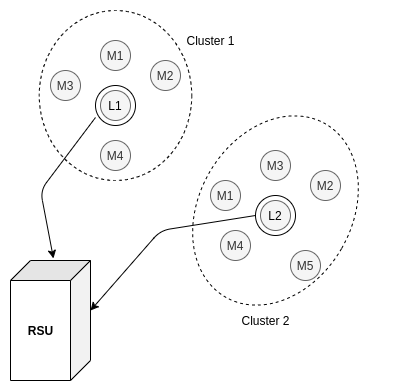
\includegraphics[scale=0.4]{Cluster.png}
    \caption{Cluster-1 with Leader $L_1$ and member nodes $M_1$ to $M_4$. Same goes for Cluster-2.}
    \label{fig:cluster}
\end{figure}

\begin{center}
    \emph{Clustering}
\end{center}
Let there be a total of $M$ clusters, each of size $k$. Then, leader
node of the cluster collects the message packets from the members
nodes and calculates the following (except his own packet) for
cluster $j$ :
\begin{enumerate}
    \item Check if $tt_i$ lies within $ET_i$, else drop the packet.
    \item Leader node computes:\\ \\
    $ h_i = H_2(M_i \: , \: tt_i \:, U_i) \:,\: \:  \: \: \: V^m_j = \sum\limits_{i=1}^{k-1} V_i \:, \\
    X^m_j = \sum\limits_{i=1}^{k-1} h_i \cdot PID_i \:
     \: \: and \: \: \:
     U^m_j = \sum\limits_{i=1}^{k-1} U_i $\\
     These values are calculated for all member nodes only, i.e., $k-1$ values.
    \item Then \emph{Leader node} signs and sends over these values of $V^m_j$, $X^m_j$ and $U^m_j$ with its own message, i.e., \\ \\ $\big \langle V^m_j \:, X^m_j \:, U^m_j \:, M_j \:, \sigma^l_j \:, PID^l_j \: \big \rangle$ \\
    where,\\
    $\sigma^l_j = (V^l_j \:, U^l_j \:, tt^l_j)$ is signature for leader of cluster $j$.
    $M_j = (M_1 \:, M_2 \:, M_3 \:, ... , M_{k})$ is the tuple containing all message strings of \emph{Member} nodes and \emph{Leader node} \\
    $PID^l_j \rightarrow PID$ for leader of cluster $j$ \\


\end{enumerate}

\begin{center}
    \emph{Verification}
\end{center}

Then RSU takes these tuples$\big \langle V^m_i \:, X^m_i \:, U^m_i \:, M_i \:, \sigma^l_i \:, PID^l_i \: \big \rangle$ from leaders of each of $M$ clusters and computes: \\
$h_i^l = H_2(M_i^l \: ,  tt_i^l \:, U_i^l)$

$M_i^l$ (Message string for leader) should be in $M_j$ tuple sent by
each cluster.
RSU accepts the message strings if this equation holds:\\ \\
$e\: \bigg( \sum\limits_{i=1}^{M} \Big[ V_i^m + V^l_i \Big] \:,\:P \bigg) \\
= e\: \bigg( \sum\limits_{i=1}^{M} \Big[ h_i^l\cdot PID_i^l + X^m_i
+ U_i^l + U^m_i\Big] \:,\:P_{pub} \bigg)  $

\begin{center}
    \emph{Clustering (Risk-mode)}
\end{center}
Another approach can be taken when sending over the signature from $Leader node$ to RSUs. Leader collects the packets $(\sigma_i \: , M_i \:, PID_i)$ from Member nodes and computes:\\
        $h_i = H_2(m_i\:,\:tt_i\:,\:U_i)$ .
Accept the messages if equation holds \\ \\
    $e\: \bigg( \sum \limits_{i=1}^{k-1}V_i\:,\:P \bigg) = e\: \bigg( \sum\limits_{i=1}^{k-1}\Big[ h_i\cdot PID_i + U_i \Big]\:,\:P_{pub} \bigg) $ \\

If the equation holds, it collects the message packet $M_i$ of each Member node and sends over $M_j = (M_1 \:, M_2 \:, ... , M_{k})$ with just its signature.\\
In short, Leader node does the message verification step for all the Member nodes and then for its own authentication sends its signature to RSU with $M_j$, i.e, Leader sends $\big \langle PID^l_j \:, \sigma^l_j \:, M_j \big \rangle$ to RSU for verification and if it holds all the messages are accepted.\\
The issue with this approach is that there’s no direct link between Member nodes and the RSU. The RSU accepts the messages of the entire cluster as long as Leader’s signature is valid. \\Thus, if there’s a malicious user in the cluster as a Member node and if it colludes with the Leader then it should be able to deliver its message easily over to RSU.\\
However this approach gives even better time and space efficiency,
so this approach can be used in cases when the Identity of Leader
node is vetted by the TAs. For example, if the Leader node is a
vehicle related to Government agencies like Police, Hospital
services etc. And we know for sure that the Leader node won't
collude with members.

\subsection{Binary Search}
In case when the batch verification equation doesn't hold means that a signature has been tampered with, or a replay attack (using an ID that has expired), or any other form of attack on the system. We need to start an individual verification process to find out the invalid signature.\\

\begin{figure}[h]
    \centering
    \captionsetup{justification=centering}
    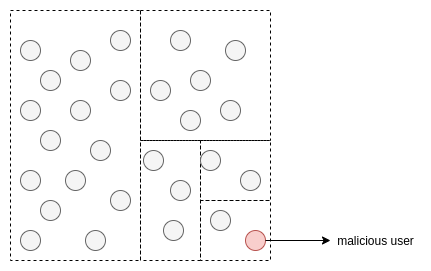
\includegraphics[scale=0.4]{binary_grey.png}
    \caption{Binary Search for malicious user.}
    \label{fig:binary_Search}
\end{figure}

We propose an idea to bring down this O(n) complexity of individual search for n-vehicles.\\
%\begin{algorithm}[h]
%\SetAlgoLined
%  \SetKwFunction{FMain}{binarySearch}
%  \SetKwProg{Fn}{Function}{:}{}
%  \Fn{\FMain{$\mathbb{S}$}}{
%        $N = $ size$(\mathbb{S})$ \\
%        \eIf{$N == 1$}{
%   bool $single\_verify = Verify(\mathbb{S})$\\
%   \If{$single\_verify ==$ false}{ \KwRet $\mathbb{S}$}
%
%   }{
%   bool $i = Batch\_Verify(\mathbb{S})$ \\
%   \eIf{$i == false$}{
%    $A = [i_0 , i_1 ….. i_{N/2}]$ elements of $\mathbb{S}$ , and \\
%    $B = [i_{N/2+1} , i_{N/2 + 2} ……. i_N]$ of $\mathbb{S}$.\\
%var $\mathbb{X} = binarySearch(A)$;\\
%\If{$\mathbb{X}$ == null} { $\mathbb{X} = binarySearch(B$);
%
%}
%\KwRet $\mathbb{X}$;
%   }
%   {
%   \KwRet $null$}
%  }
%  }
%\caption{Binary Search}
%\end{algorithm}

\section{RHA Scheme : \emph{RSU-to-Vehicle}}
We remove the \emph{Pseudo-ID generation} part, rest is the same as
Vehicle-to-RSU in our scheme.


\subsection{Private Key Extraction}
 \begin{enumerate}

     \item PKG computes the private key $\xrightarrow{} XID_R = s \cdot RID_R$, given $RID_R$ is the real-ID of a RSU and $s$ is the master-secret key for PKG.
     \item PKG sends $XID_R$ to vehicle over a trusted network. Then RSU stores $XID_R$ corresponding to $RID_R$.
 \end{enumerate}

\subsection{Message Signing}
\begin{enumerate}
    \item Vehicle uses $RID_R$ from storage and a random $r_i \in \mathbb{Z}/q$
    \item Vehicle calculates $h_i = H_2(m_i\:,tt_i \: , U_R)$ and $U_R = r_i \cdot RID_R$
    \item Vehicle computes $V_R = (r_i+h_i) \cdot XID_R$
    \item Vehicle calculates signature $\sigma_i = (U_R\:,\:V_R\:,\:tt_i)$
    \item Vehicle sends a tuple of  $\langle\sigma_i \: , \: m_i , \: RID_R\rangle$ to the RSU
\end{enumerate}

\subsection{Message Verification}
\begin{enumerate}
    \item Check whether $tt_i$ lies in $ET_i$ i.e the time limit for the ID hasn't expired.
     \item Compute $h_i = H_2(m_i\:,\:tt_i\:,\:U_R)$ for packet
    \item Verify whether the following condition holds or not. $$e(V_R\:,\:P) = e(h_i\cdot RID_R + U_R\:,\:P_{pub}) $$.
\end{enumerate}
If it holds accept message signature.

\subsection{Batch Verification}
\begin{enumerate}
    \item Discard all the frames for which $tt_i$ doesn't lie in $ET_i$
    \item Compute $h_i = H_2(m_i\:,\:tt_i\:,\:U_R)$ for each packet
    \item Accept the entire batch if this holds \\
    $$e\:\Bigg( \sum_{i=1}^{n}V_R\:,\:P \Bigg) = e\:\Bigg(\sum_{i=1}^{n} \big[ h_i\cdot RID_R + U_R \big]\:,\:P_{pub} \Bigg) $$
\end{enumerate}


\section{Security Analysis}
\subsection{Source Authentication and Message Integrity}
We show that our scheme is \emph{euf-cma} (existentially unforgeable under an adaptive chosen-message attack) in the random oracle model under \emph{CDH assumption}. \\ \\
\emph{Proof} : Suppose \emph{A} is a forger who breaks our scheme.
Algorithm \emph{B} is given a ECDLP instance $(P ,\: XID \cdot P)$.
Let $Q$ and $R$ be the number of queries that an algorithm $A$ can
ask the random oracle and the number of queries that $A$ can ask to
sign the oracle, respectively. By using \emph{A} we will construct
an algorithm \emph{B} that breaks ECDLP and outputs $XID$ given $(P
,\: XID \cdot P)$ within a time period $T$ which is expected to be
less
than $120686\cdot QT/\varepsilon$, if $\varepsilon\: \geq\: 10(R+1)(R+Q)/q$. $B$ performs the following simulation by interacting with $A$. At anytime, $A$ can query the random oracles $H_1$ and $H_2$ , Extract , ID-Sign Oracle. \\

\noindent\emph{Setup} : Algorithm $B$ sets $P_{pub} = sP$ and starts by giving $A$ the system parameters $Params$, including $\langle P, P_{pub} \rangle$.\\

\noindent\emph{$H_1$ and $H_2$ queries} : To respond to $H_1$
queries ($H_2$ queries), $B$ maintains a list of tuples $(RID , ET ,
PID) \:\: ((M , U , h))$ . We refer to this list as the $H_1$-list
($H_2$-list). When A queries the oracle $H_1\:(H_2)$ at $(RID \:,
\:ET)\:\:((M\:,\:U))$ , B responds as follows.
\begin{enumerate}
    \item If the query $(RID\: , \: ET)\:\:((M\:,\:U))$ already appears on the $H_1$-list ($H_2$-list) in a tuple $(RID\: , \:ET \:, \:PID)\:\:((M\:,\:U\:,\:h))$ then B responds with $H_1(RID\:,\:ET) = PID\in \mathbb{G}_1$\:\:\:\\$(H_2(M\:,\:U)\:=\:h \in Z_q)$
    \item Otherwise, B picks a random $PID \in \mathbb{G}_1 \:\:\:(h\in Z_q)$, adds tuple $(RID , ET , PID)\:\:\: ((M\:,\:U\:,\:h))$ to the $H_1$-list ($H_2$-list) and responds to A with \\
    $H_1(RID , ET) = PID$\:\:\:$(H_2(M\:,\:U) = h)$ \\
\end{enumerate}

\noindent\emph{Extract (Pseudo-ID/Private Key) query} : When A queries a private key corresponding to $RID_i$. Then B responds to A with $(PID\:,\:XID)$ where, $XID = s \cdot PID$ and stores $(RID\:,\:PID\:,\:XID)$ to the Ext-list.\\
At any time, A can query the signing oracle. To answer these queries B does the following.\\

\noindent\emph{Sign Queries} :  When A makes an ID-sign query on M for $RID$ , B finds $(RID\:,\:PID\:,\:XID)$ from the ext-list.\\
B computes $h$ = $H_2\:(M\:,tt_i\:,\:U) \in Z_q$ where $U$ = $r\cdot PID$ and $V = (r+h)\cdot XID$, for a random $r \in \mathbb{Z}_q$\\

Then, $\sigma = (U\:,\:V\:,\:tt)$ is a valid signature on M, since
it satisfies $e(h\cdot PID + U\:,\: P_{pub})  = e((r+h)\cdot XID
\:,\:P) = e(V\:,\:P)$
\begin{itemize}
    \item If $(RID\: , \:PID\: , \:XID)$ already appears on the Ext-list, then B can compute a signature $\sigma$ by performing the signing algorithm.
    \item Otherwise, B requests an extract-query to obtain the corresponding private key $XID$. Then, B computes a signature $\sigma$ on M for $PID$ using $XID$ , repsonds to A with $\sigma$ and stores $(RID\:,\:PID\:,\:XID)$ to Ext-list.
\end{itemize}
Note that A's view is identical to it's view in the real attack.\\

\emph{Output} : By forking lemma, after replaying A with the same
random tape, B obtains two valid signatures $\sigma = (M^*\:,\:
h\:,\:  U \:,\:  V)$ and $\sigma' = (M^* \:,\: h^* \:,\: U \:,\:
V^*)$ within a polynomial time, where $V = (r+h)\cdot XID$ , $V^* =
(r+h^*)\cdot XID$. Then B computes
\begin{equation}
    \displaystyle \frac{h^* \: V \:-\: h \: V^*}{r\cdot(h^*\: -\: h\:)} = XID
\end{equation}

We can achieve $XID$ as solution to the ECDLP instance, within an
expected time less than $120686\cdot QT/\varepsilon$, if
$\varepsilon\: \geq\: 10(R+1)(R+Q)/q$.


\subsection{Resistance to replay attack}
A current timestamp $tt_i$ is attached to messages in our scheme
$h_i = H_2(m_i\:,tt_i \: , U_i)$. \\
$ET_i$ is the validity period for a Pseudo-ID of a vehicle. We check
if $tt_i$ lies within $ET_i$ , in which case we accept the message.
Otherwise, we drop it.

\subsection{Traceability}
Given a pseudo-ID $PID$ in a signed message, the TRA with the master
secret $\alpha$ for traceability can trace the real identity of a
vehicle by computing $PID$.

\subsection{Role Separation}
Both TA’s (TRA and PKG) have their separate role assigned. TRA
generates Pseudo-IDs for vehicles and PKG gives Private keys for
these corresponding IDs. Only TRA with tracing secret key $\alpha$
can trace the RID (Real Identity of Vehicle). This role separation
helps making sure there’s no concentration of power(leads to
single point of failure).

\subsection{Short Term Linkability}
A malicious user may try to act as different vehicles, known as
Sybil\cite{r4} attack, and can be countered by Short-term
linkability. Unless the Pseudo-ID for a vehicle expires (i.e. ET,
validity period, is over), all the message signed with the same PID
can be recognised by RSUs. This doesn't lead to invasion of privacy
but these messages from the malicious user can be dropped. So if a
vehicles transmits multiples messages within a time frame of ET the
nearest RSU will recognise this behaviour and drop these messages
from its buffer.

\subsection{Long term unlinkability}
In our scheme, different messages are signed by different
Pseudo-IDs. A pseudo-ID expires after ET (its validity period)
passes. So, if the same vehicle sends over another message packet
after ET time, then it won’t be possible for any adversary to find
out the RID(real ID) of the vehicle from PID (Pseudo-ID).




\section{Performance Analysis}
\label{L7}

\subsection{Time Analysis}
\label{L72}

\begin{table*}[]
\centering
\caption{Time Analysis}
\begin{tabular}{|c|c|c|c|c|}
\hline Scheme &
  \begin{tabular}[c]{@{}c@{}}Pseudo ID generation/\\ Private Key Generation\end{tabular} &
  \begin{tabular}[c]{@{}c@{}}Message \\ Signing\end{tabular} &
  \begin{tabular}[c]{@{}c@{}}Message \\ Verification\end{tabular} &
  \begin{tabular}[c]{@{}c@{}}Batch \\ Verification\end{tabular} \\ \hline
\emph{RHA} (Our scheme) &
  \begin{tabular}[c]{@{}c@{}}$T_{mp}$ + $T_{hf}$ =\\ 0.3001 ms\end{tabular} &
  \begin{tabular}[c]{@{}c@{}}$2*T_{mp} + T_{hf}$ =\\ 0.6001 ms\end{tabular} &
  \begin{tabular}[c]{@{}c@{}}$T_{hf} + T_{mp}$ + \\$T_{pa-mp} + 2*T_{bp}$ \\ = 5.2501 ms\end{tabular} &
  \begin{tabular}[c]{@{}c@{}}n * $T_{hf} + n*T_{mp}$ \\+ $(3n-2)*T_{pa-mp}$ + $2*T_{bp}$\end{tabular} \\ \hline
Shim's Scheme \emph{(CPAS)}\cite{r1} &
  \begin{tabular}[c]{@{}c@{}}4* $T_{mp} + 2*T_{hf}$ =\\ 1.2002 ms\end{tabular} &
  \begin{tabular}[c]{@{}c@{}}$T_{mp}$ + $T_{pa-mp}$ + $T_{hf}$ =\\ 0.6701 ms\end{tabular} &
  N/A &
  \begin{tabular}[c]{@{}c@{}}2n*$T_{hf}$+ (n+1)*$T_{mp}$ +\\ (3n-3)*$T_{pa-mp}$ + 3*$T_{bp}$\end{tabular} \\ \hline
\begin{tabular}[c]{@{}c@{}}Zhang et al.’s\\ Scheme\cite{r13}\end{tabular} &
  \begin{tabular}[c]{@{}c@{}}3* $T_{mp} + T_{pa-mp} + 2*T_{hf}$ =\\ 1.2702 ms\end{tabular} &
  \begin{tabular}[c]{@{}c@{}}3*$T_{mp} + T_{mtp} + T_{pa-mp}$\\ $+ 2*T_{hf} $ =\\ 1.3402 ms\end{tabular} &
  \begin{tabular}[c]{@{}c@{}}2*$T_{hf} + T_{pa-mp}$\\ + $2*T_{mp} + 3*T_{bp}$\\ = 9.9402 ms\end{tabular} &
  \begin{tabular}[c]{@{}c@{}}3*$T_{bp}$ + \\ (n+1)*$T_{mp}$ + \\ (3n-2)*$T_{pa-mp}$ + \\ 3n*$T_{hf}$\end{tabular} \\ \hline
\begin{tabular}[c]{@{}c@{}}Bayat et al.’s \\ Scheme\cite{r3}\end{tabular} &
  \begin{tabular}[c]{@{}c@{}}$3*T_{mp} + T_{pa-mp} + T_{hf} $ =\\ 1.2701 ms\end{tabular} &
  \begin{tabular}[c]{@{}c@{}}2*$T_{mp} + T_{pa-mp} + T_{hf} + T_{mtp}$ =\\ 1.0401 ms\end{tabular} &
  \begin{tabular}[c]{@{}c@{}}3* $T_{bp} + T_{pa-mp}$\\ +$ T_{hf} + T_{mtp}$ =\\ 9.4101 ms\end{tabular} &
  \begin{tabular}[c]{@{}c@{}}3*$T_{bp}$ + (3n-3)*$T_{pa-mp}$ + \\ n*$T_{hf}$ + n*$T_{mtp}$\end{tabular} \\ \hline
%caption{Table for Time analysis comparative study}
\end{tabular}
\end{table*}

\begin{figure}[h]
    \centering
    \captionsetup{justification=centering}
    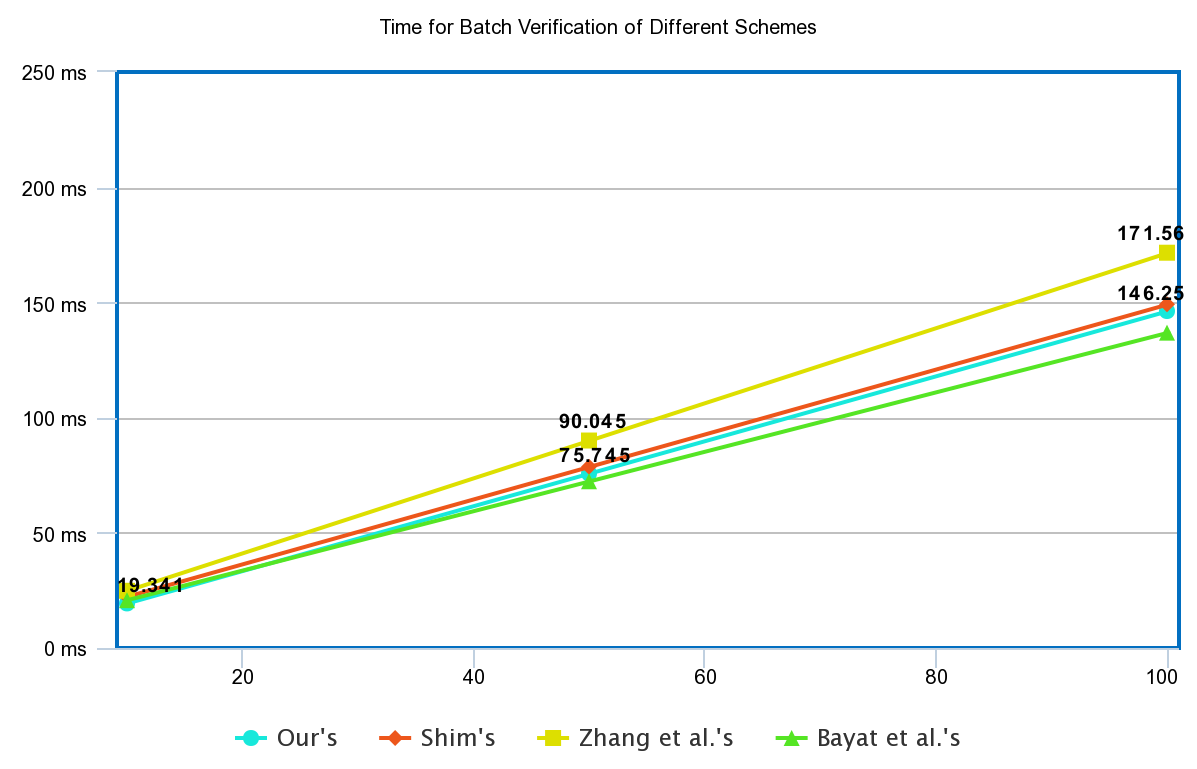
\includegraphics[scale=0.2]{batch.png}
    \caption{Comparison study of batch verification time for various schemes }
    \label{fig:Batch_Verify}
\end{figure}




% \begin{tikzpicture}
% \begin{axis}
% [xlabel={Number of messages},ylabel={Time}]
% \addplot [
% domain= 10:100,
% samples=100,
% color=black,
% ]
% {x*0.0001+x*0.3 +(3*x-2)*0.37 +2*2.99};
% \addlegendentry{RHA}

% \addplot [
% domain= 10:100,
% samples=100,
% color=red,
% ]
% {2*x*0.0001+(x+1)*0.3 +(3*x-3)*0.37 +3*2.99};
% \addlegendentry{Shim}

% \addplot [
% domain= 10:100,
% samples=100,
% color=yellow,
% ]
% {3*x*0.0001+(x+1)*0.3 +(3*x-2)*0.37 +3*2.99 +2*x*0.106};
% \addlegendentry{Zhang}

% \addplot [
% domain= 10:100,
% samples=100,
% color=blue,
% ]
% {x*0.0001+(3*x-3)*0.37 +3*2.99 +x*0.0106 +x*0.07};
% \addlegendentry{Bayat}
% \end{axis}
% \end{tikzpicture}
% \caption{Time for Batch Verification of different schemes}
% \label{fig:Batch_Verify_Time}





\begin{figure}[h]
    \centering
    \captionsetup{justification=centering}
    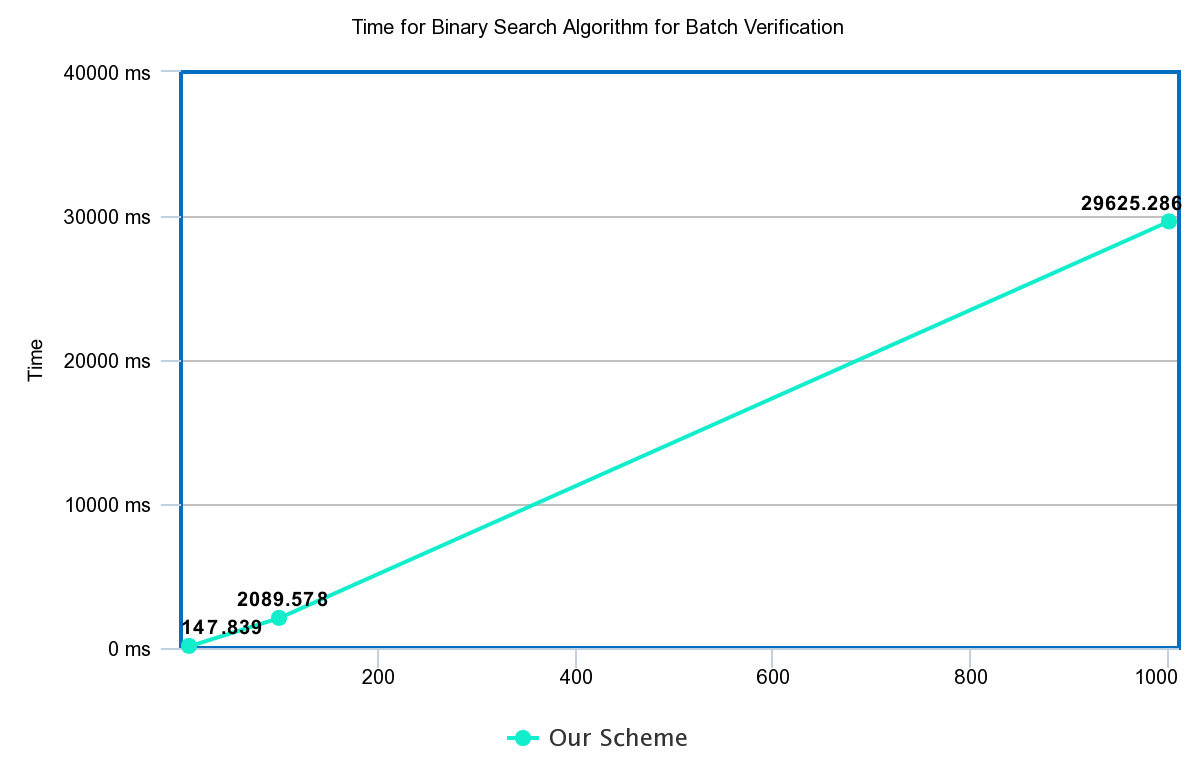
\includegraphics[scale=0.2]{bin.png}
    \caption{Time for Binary Search. Worst time complexity being $1 + 2 \log_2(n)[f(n)]$ }
    \label{fig:Binary_Search_Time}
\end{figure}


For our scheme, we have used the MIRACL library and chosen a 160-
bit elliptic curve for our scheme. All performance results have been
calculated by using that library on our specific system. In case of
time analysis, we divide the scheme into individual operations and
calculate the time for each operation. The program is run for 10
seconds (10,000 ms) and in that time the number of iterations are
recorded for every operation and from that we obtain the time. For
comparison purposes, we categorize the operations into mainly 6
parts:
\begin{enumerate}
\setlength\itemsep{0.65em}
    \item the execution time of a scalar multiplication operation $x\cdot P$, related to the bilinear pairing, where $x\in \mathbb{Z}_q^*$ and $P \in \mathbb{G}_1$ (33,046 iterations) \\ $T_{mp} = 0.30 ms$
    \item The execution time for point addition of 2 scalar multiplication of 2 points on the curve (Ex. $x\cdot P + y\cdot Q$, where x and y are scalars and $P,Q \in \mathbb{G}_1$) (27,023 iterations)\\
    $T_{pa-mp} = 0.37 ms$
    \item The execution time of a bilinear pairing operation $e(S,T)$ , where $S,T \in \mathbb{G}_1$ (3,341 iterations)\\
    $ T_{bp} = 2.99 ms$
    \item The execution time of a hash function ($T_{hf}$). Most standard cryptography hash functions take negligible time (ex. SHA-1), unless it is MaptoPoint Hash function but we will consider it as 0.0001 ms.
    \item Execution time of a map-to-point hash function (142386 iterations)\\
    $T_{mtp} = 0.07ms$
    \item The execution time of a small-scale multiplication operation $v_i \cdot P$
related to the bilinear pairing where $P \in \mathbb{G}_1$ , $v_i$ is a small random integer in $[1,2^t]$ and $t$ is a small integer (94,335 iterations)\\
$T_{mp-s}$= 0.106 ms
\end{enumerate}
All these times are calculated in Intel Core i5-7200U CPU @2.5 GHz
up to 2.7 GHz, 8 GB RAM and 64-bit OS and x64 based processor
(Rohan’s system). We draw comparison with three other VANET
schemes (Shim\cite{r1}, Zhang et al.\cite{r13} and Bayat et
al.\cite{r3}) based on bilinear pairings in order to understand how
much of an improvement our scheme is in terms of time efficiency.

\begin{figure}[h]
    \centering
    \captionsetup{justification=centering}
    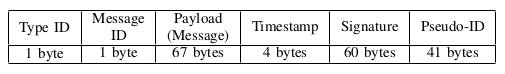
\includegraphics[scale=0.5]{space.png}
    \caption{Study of Space taken by various schemes}
    \label{fig:Space_Taken}
\end{figure}


\subsection{Communication overhead}
The communication overhead of the proposed scheme is discussed as
follows. In order to reduce signature size, Shim\cite{r1} developed
a method to reduce the size of a point Q = (x, y) if an OBU or an
RSU can send this point to a well- designed destination, i.e.,
another RSU or OBU. The signature size reduction method is that an
OBU or an RSU only sends the x- coordinate of Q and the designed
destination can learn the y- coordinate by computing the square
root. Since the size of the signature is reduced by applying
Shim’s method, the total communication cost of CPAS is reduced.
Table above shows the format of the signed message adopted in our
scheme. Based on the same signature size reduction method, since our
scheme uses 160- bit subgroup Elliptic Curve instead of a 159-bit
subgroup of the MNT curve with an embedding degree of 6 is used in
Shim’s scheme, the total size of one signed message is 160 + 160 +
160 + 3 = 483 bits = 60.375 bytes. Then, the total size of pseudo ID
is 160 + 160 + 2 + 4 = 326 bits = 40.75 bytes, where the timestamp
field is set as 4 bytes. Hence, the total message size from vehicle
(OBU) to RSU in the proposed authentication scheme is only 174 bytes
based on the signed message format shown in the table above. If the
size reduction method proposed by Shim\cite{r1} is adopted, our
proposed scheme has the same signature size as CPAS. In summary, the
proposed scheme and CPAS require less communication bandwidth to
transmit signed messages by applying the signature size reduction
method and corresponding message format when comparing with signed
messages using current IEEE Trial-Use standard format for VANET
security (which takes a total of 250 bytes per signed message).


\section{Conclusion}
\label{L8}We have proposed a secure conditional privacy-preserving
authentication scheme using a new IBS scheme with the one of the
fastest batch verification process for secure V-to-I communications
in VANETs. The scheme achieves conditional privacy preservation in
which each message launched by a vehicle has been mapped to a
distinct pseudo-ID and a TRA can always retrieve the real identity
of a vehicle from any pseudo-ID.

In the scheme, an RSU can simultaneously verify multiple received
signatures such that the total verification time can be considerably
reduced. We have also proposed two methods to significantly increase
the efficiency of batch verification. It is common for all VANET
schemes to include batch verification but no one considers that it
is a waste to discard all the messages in the batch just because one
of the message signatures doesn’t check out. Ours is the first
scheme in that regard to propose a less wasteful (in terms of data)
solution to fix this.

Although our scheme has covered and solved most of the common
attacks in networks, there is still room for improvement. A recently
emerging form of attack is DDOS (Distributed Denial of Service),
which is when the hackers decide to jam the network with unnecessary
data packets so legitimate users cannot use the network to
communicate. It is done in a distributed manner, i.e. thousands of
computer systems run by bots are involved in such an attack and so
it is impossible to identify who is a legitimate user and who is a
malicious user.

There are a few solutions to solve this problem although not
implemented in our scheme. One, we could set up a DDOS challenger
similar to an Adversary challenger which will ask every user and so
even the botnet to solve few puzzles only a human can solve and
hence they will be caught. Second, we could use machine learning
algorithms to monitor the number of messages being sent from a
vehicle and try to find the botnet systems in that way and stop
their access. Third, and possibly the surest way to stop these
botnets is the IP Reputation. DDOS attacks happen in every server
every network and they are monitored and their IP’s are noted so
in future no other server is affected by it. So, we simply block all
the IP’s that have a bad IP reputation. In terms of performance,
our scheme is on par and better than some of the recently developed
schemes in VANET authentication in all three respects of time, space
and security analysis.

In terms of what some additional problems that remain to be solved
in the future is the localised databases of the RSUs. The RSU
whether a vehicle is registered and legitimate but when the vehicle
crosses the range of coverage of that particular RSU and heads into
the territory of an RSU, it doesn’t recognize it. The obvious
solution would be to have a common database of all the vehicles
registered under the VANET scheme, and load that database onto every
RSU, which is a immense waste of space. A better solution to this
remains to be discovered in the future.


\bibliographystyle{ieeetran}
\bibliography{harsvanet}


\end{document}
